% The two lanes of section 7: what the compiler can do before the run, and
% what only the run can answer. The paper's measurement contribution is the
% arrow between them -- the compiler emits a TABLE, not a verdict -- and that
% is the thing to look at.
%
% Colour is not load-bearing: the two lanes are told apart by position and by
% their dashed enclosures, and the handoff arrow is the one accent.
%
% WIDTH. \textwidth is 395.8pt; keep this under ~385pt.
%
%   make figures                              compiles it
%   \includegraphics{figures/two-lane}        includes it
\documentclass[tikz,border=3pt]{standalone}
% ---------------------------------------------------------------------------
% figures/house.tex -- the shared look. Every figure \input's this, so six
% figures look like one hand drew them instead of six.
%
% HOW FIGURES WORK HERE. tikz/pgf is NOT on ACM's production package list, so
% the documents never load it. Each figure is its own standalone document in
% this directory, compiled to a PDF by `make figures`, and pulled into a
% section with
%
%     \begin{figure}
%       \centering
%       \includegraphics{figures/my-figure}
%       \caption{What to LOOK at, not what the figure is of.}
%       \label{fig:my-figure}
%     \end{figure}
%
% Three conventions:
%   * a float sits where it is discussed;
%   * a caption says what to look at, not what the figure is of;
%   * a figure is checked by rendering it and looking, not by a clean compile.
%
% The palette below is the same as the one in preamble.tex. It is repeated
% rather than shared because these are standalone documents that never see the
% paper's preamble, so a colour changed there must be changed here too.
% ---------------------------------------------------------------------------
\usepackage{amsmath}
% The figures build with LuaLaTeX like the documents, so their text is the
% paper's Libertine and their code is the paper's Iosevka.
\usepackage{fontspec}
\setmainfont{LinLibertine_R.otf}[BoldFont=LinLibertine_RB.otf,ItalicFont=LinLibertine_RI.otf,BoldItalicFont=LinLibertine_RBI.otf,Ligatures=TeX]
\setmonofont{Iosevka Custom}[Scale=MatchLowercase,RawFeature={-liga,-calt,-clig,-dlig}]
% Math in the figures is the paper's math: acmart sets Libertinus Math under
% LuaTeX, so the letters on a wire match the letters in the text around it.
\usepackage{unicode-math}
\setmathfont{LibertinusMath-Regular.otf}
\usetikzlibrary{positioning,arrows.meta,fit,backgrounds,calc}

% Blackboard Z, which the documents get from the paper preamble.
% Kept here so a figure never reaches for the paper's preamble.
\newcommand{\Z}{\mathbb{Z}}


\definecolor{ink}{HTML}{16191D}
\definecolor{accent}{HTML}{1F4E79}
\definecolor{accentsoft}{HTML}{E8EEF4}
% accent, accentwarm and accentplum mark the temporary's basis level -- level
% 0, 1, 2 -- wherever a picture or a matrix has to show which branch is which.
\definecolor{accentwarm}{HTML}{9A5B00}
\definecolor{accentplum}{HTML}{8E2F5F}
\definecolor{muted}{HTML}{5B6470}
\definecolor{hairline}{HTML}{C9CFD6}

\tikzset{
  % Every figure inherits this: thin lines, small type, generous air.
  house/.style={
    >={Stealth[length=2.1mm, width=1.6mm]},
    line width=0.5pt,
    node distance=9mm and 15mm,
    every node/.style={font=\small},
  },
  % A thing.
  box/.style={
    draw=ink, line width=0.5pt, rounded corners=1.5pt,
    inner xsep=6pt, inner ysep=4pt, align=center,
  },
  % A thing we are drawing attention to. One per figure, at most.
  boxhi/.style={box, draw=accent, fill=accentsoft, text=ink},
  % A thing that is context, not content.
  boxdim/.style={box, draw=hairline, text=muted},
  % An arrow, and the word on it.
  flow/.style={->, draw=ink},
  flowdim/.style={->, draw=hairline},
  lbl/.style={font=\footnotesize\itshape, text=accent, inner sep=2pt},
  lbldim/.style={font=\footnotesize, text=muted, inner sep=2pt},
  % A dashed grouping rectangle behind a set of nodes.
  group/.style={draw=hairline, dashed, rounded corners=2pt, inner sep=7pt},
}


\begin{document}
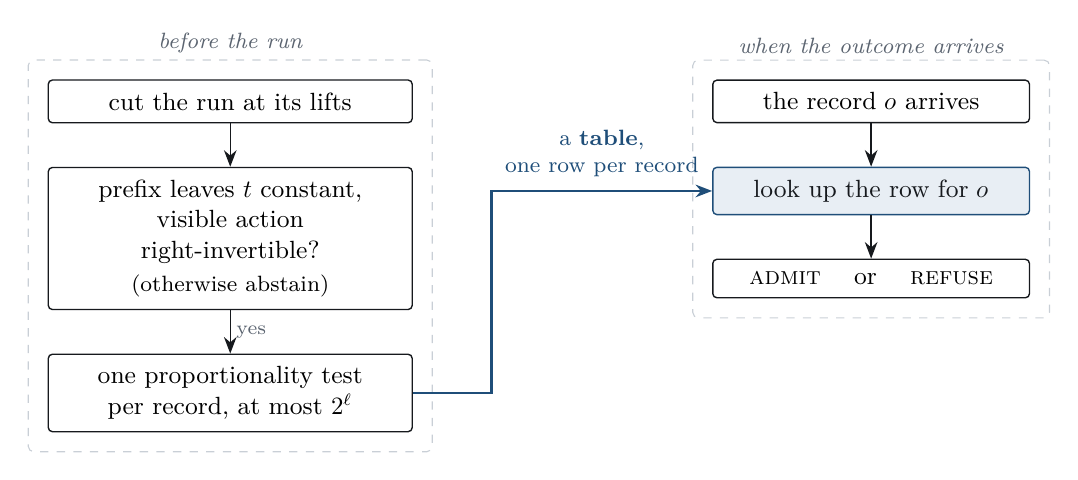
\begin{tikzpicture}[house, node distance=5.5mm and 10mm]

  % ---- left lane: before the run --------------------------------------
  \node[box, text width=42mm, inner ysep=4.5pt] (cut)
    {cut the run at its lifts};
  \node[box, below=of cut, text width=42mm, inner ysep=4.5pt] (const)
    {prefix leaves $t$ constant,\\visible action right-invertible?\\[1pt]
     \footnotesize (otherwise abstain)};
  \node[box, below=of const, text width=42mm, inner ysep=4.5pt] (test)
    {one proportionality test\\per record, at most $2^{\ell}$};

  \draw[flow] (cut) -- (const);
  \draw[flow] (const) -- node[lbldim, right, font=\scriptsize] {yes} (test);

  % ---- right lane: when the outcome arrives ---------------------------
  \node[box, right=38mm of cut, text width=36mm, inner ysep=4.5pt] (rec)
    {the record $o$ arrives};
  \node[boxhi, below=of rec, text width=36mm, inner ysep=4.5pt] (look)
    {look up the row for $o$};
  \node[box, below=of look, text width=36mm, inner ysep=4.5pt] (verdict)
    {\textsc{admit} \quad or \quad \textsc{refuse}};

  \draw[flow] (rec) -- (look);
  \draw[flow] (look) -- (verdict);

  % ---- the handoff: a table, not a verdict ----------------------------
  \draw[->, draw=accent, line width=0.9pt]
    (test.east) -- ++(10mm,0) coordinate (bend) |- (look.west);
  % Centred on the horizontal run it names, clear of the lane boundary.
  \node[font=\footnotesize, text=accent, align=center, inner sep=1pt,
        anchor=south]
    at ($(bend |- look.west)!0.5!(look.west) + (0,1.4mm)$)
    {a \textbf{table},\\one row per record};

  \begin{scope}[on background layer]
    \node[group, fit=(cut)(test),
          label={[lbldim, font=\footnotesize\itshape]above:before the run}] {};
    \node[group, fit=(rec)(verdict),
          label={[lbldim, font=\footnotesize\itshape]above:when the outcome arrives}] {};
  \end{scope}

\end{tikzpicture}
\end{document}
